
% Emerging TF
\section{Emerging Transcription Factors} \label{s:N_I:sel_tfs}

% Introduce the motivation of using TF
After comparing the two community detection algorithms and selecting SBM, it is important to delve into the analysis of the network output. Previous work in this thesis demonstrated that allowing a higher minimum degree for a specific subset of TF affects the graph metrics and community detection methods. However, in the network pipeline, not all the genes used to generate the graph are employed for cancer stratification; instead, the top 100 genes are selected by ModCon (see \cref{fig:N_I:network_pipeline}). It is important to remember that the ModCon score considers a node’s degree, its edge weights, as well as the median expression and dispersion of the gene in the dataset used to build the network; see \cref{s:N_I:methods_modcon} for a more detailed description.


\begin{figure}[!b]   
    \centering
    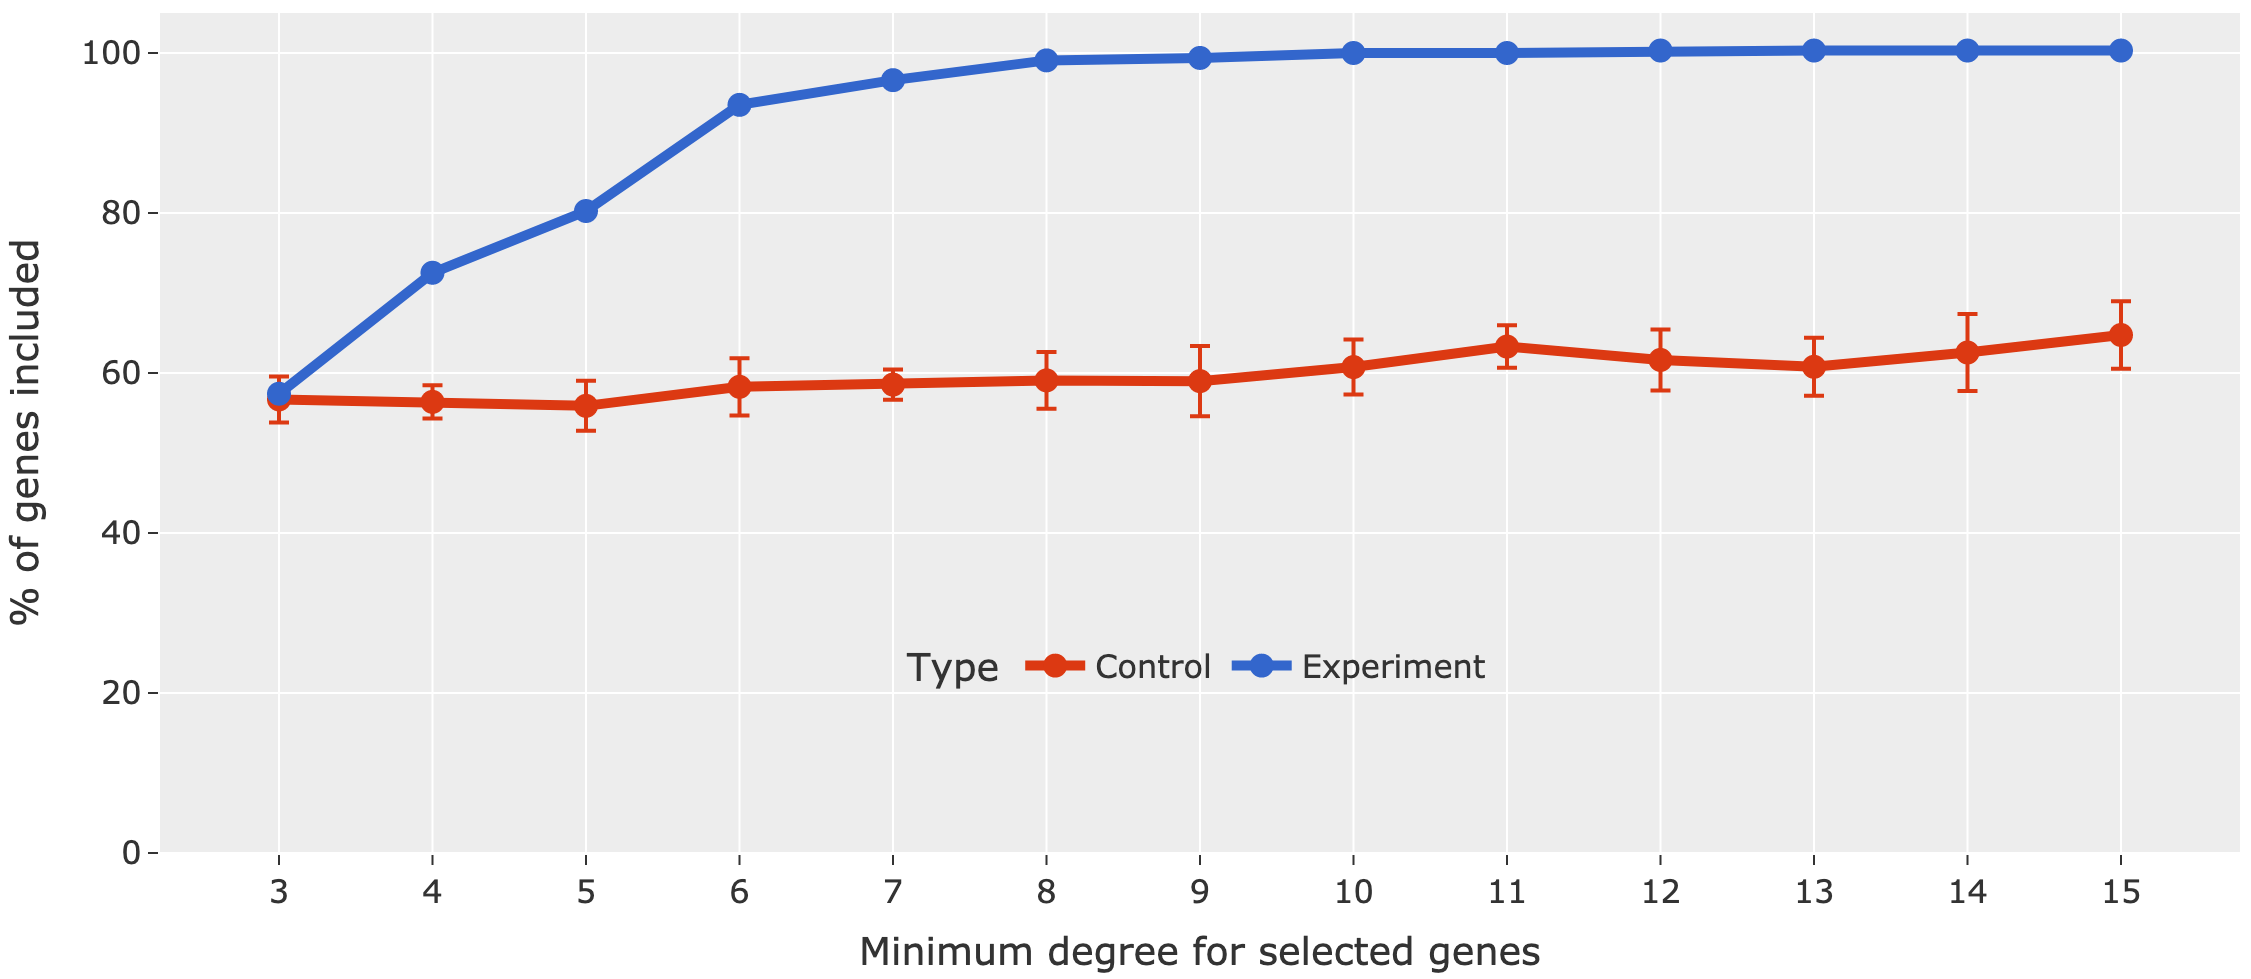
\includegraphics[width=1.0\textwidth,height=1.0\textheight,keepaspectratio]{Sections/Network_I/Resources/selective_pruning/com_comp/ctrls_min_dig_mev.png}
      \caption[Community detection performance in selective edge pruning]{The percentages of the Transcription Factors selected by ModCon from the communities found with \gls{SBM} as the minimum degree increases. By having $\sim60\%$ of the Transcription Factors selected by ModCon the plot shows there is a subset of TF that are 'naturally' highly correlated with other genes. It also shows that the biggest effect on the ModCon score is when the minimum degree for TF is set to 6.}
    \label{fig:N_I:sel_tfs}
\end{figure}

% Presentin the Graph of sel TF-s. 
% -- all TF are included when minimum degree is set to 15 and there is no added benefit when TF = 6
\Cref{fig:N_I:sel_tfs} show the percentages of the TF genes (325 in total) that are selected by the ModCon score to stratify the disease. SBM community detection was used with both selected genes that are TF and non-TF 325 genes as control, the latter was run 10 times.

There is a clear difference between the Experiment and the Control traces, where the genes in the Experiment, with a real biological value, gradually increase with the minimum degree values, while the controls remain at a similar level of $\sim60\%$. All the TF genes are included when the minimum degree of a TF reaches to 15 and the biggest percentage included after TF passes minimum degree of 6. For this reason and that the SBM performance is affected as the minimum degree increase, the value of 6 for the minimum number of edges was chosen for selective edge pruning.


% Biological relevance
% -- Because 50% of the TF naturally emerges and used for subtyping
In contrast to the Experiment trace, the Control appears to have a constant number of biological TF selected by ModCon, of $\sim60\%$. This means that there is a subset of TF which are consistently selected by ModCon (i.e. with a high connectivity) despite other than 325 TF were allowed a high number of connections. To explain this behaviour, it is worth re-surfacing the selective edge pruning process. For each gene in the correlation matrix only the 3 highest correlated genes are kept for standard genes or 6 for the selected genes to prioritise. Thus, a gene can have a starting degree either of 3 or 6. For a node $A$ to have higher a degree, it needs that other genes to have node A in their top correlation. For example, if node $A$ is a non-TF gene and it has a degree value of 10, it means that 7 other genes have node $A$ in their top correlations. This means that the  $\sim60\%$ of TF from the control experiment have a high connectivity score through their neighbours.

% Biological significance
Taking in account the selective edge pruning and that $\sim60\%$ of the 325 TF genes are selected by ModCon, when the TF are \textbf{explicitly} not prioritised, it is remarkable to have a subset of genes that emerged as being highly connected. To further refine the list, the intersection of genes across the controls is taken and this leads to a list of 98 TF, that are constantly highly connected across the controls. 

\begin{figure}[!b]   
\centering
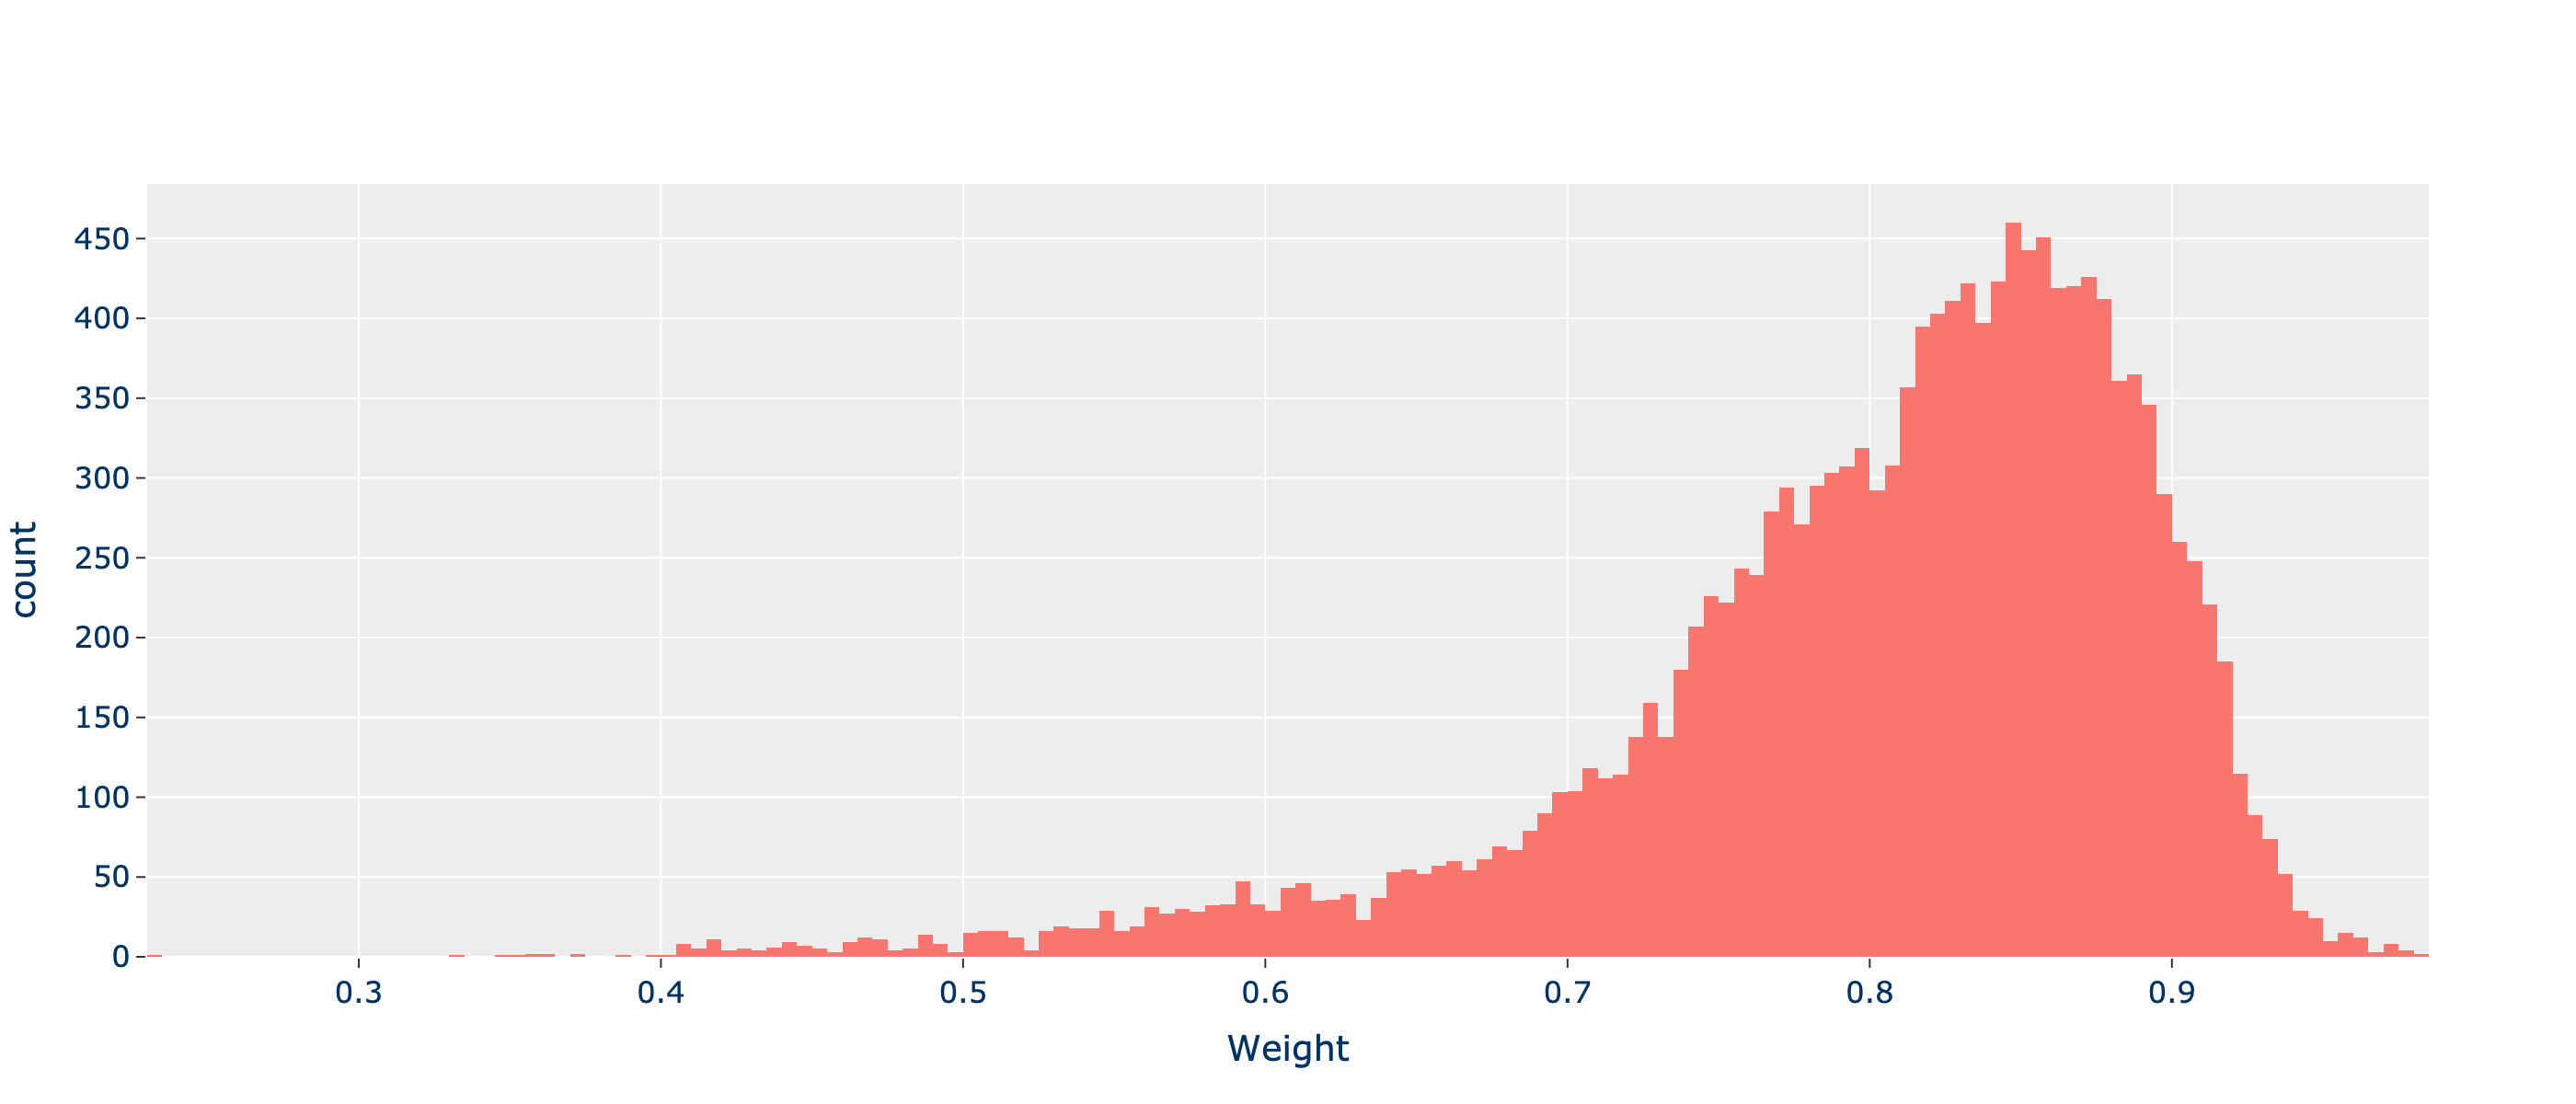
\includegraphics[width=1.0\textwidth,height=1.0\textheight,keepaspectratio]{Sections/Network_I/Resources/selective_pruning/weight_distrib.png}
  \caption[Weight distribution]{The weight distribution of the edges weights in a standard network (no weight modifier), with 3 edges for non-TF and 6 for TF genes. The distribution is skewed to the left showing that the selective edge prune keeps only the highly correlated pairs of genes with Spearman correlation over 0.5. }
\label{fig:N_I:weight_distrib}
\end{figure}

\subsubsection*{Weight distribution}

% Shows that the selective edge pruning only selects the highly correlated genes
In the selective edge pruning strategy there is no threshold to ensure that the low correlated pair of genes are not cluttering the network and that the most co-expressed pairs are kept. To test this the weight distribution is plotted in \cref{fig:N_I:weight_distrib} for a standard network with no weight modifiers, with a minimum 3 edges per standard gene and 6 per TF. It can be seen that the distribution is skewed right, ensuring that most of the genes are highly correlated.


Overall this section showed that the genes selected through ModCon are affected by the selective edge pruning. It also showed that there is a subset of 98 \acrlong{tf} that are highly correlated in the tumour dataset, which indicates their higher role in biological role. These genes are explored in more detail in the following section.


% MIBC comparison
\subsection{Subset of TF: MIBC comparison} \label{s:N_I:sel_tfs_mibc}

The analysis so far indicates that the 98 genes are a subset of TF which are highly correlated with the other genes in the network, even when other subsets of nodes are allowed a higher minimum degree. To further understand their function the tumour expression of the 98 TF is used to stratify the MIBC which resulted in five major groups, see the details of the clustering in the work from Appendix \cref{s:ap:sel_tfs_cs}.

\begin{figure}[!htb]
    \centering
    % Sankey - consensus and K-means comparison
    \begin{subfigure}[!t]{1.0\textwidth}
        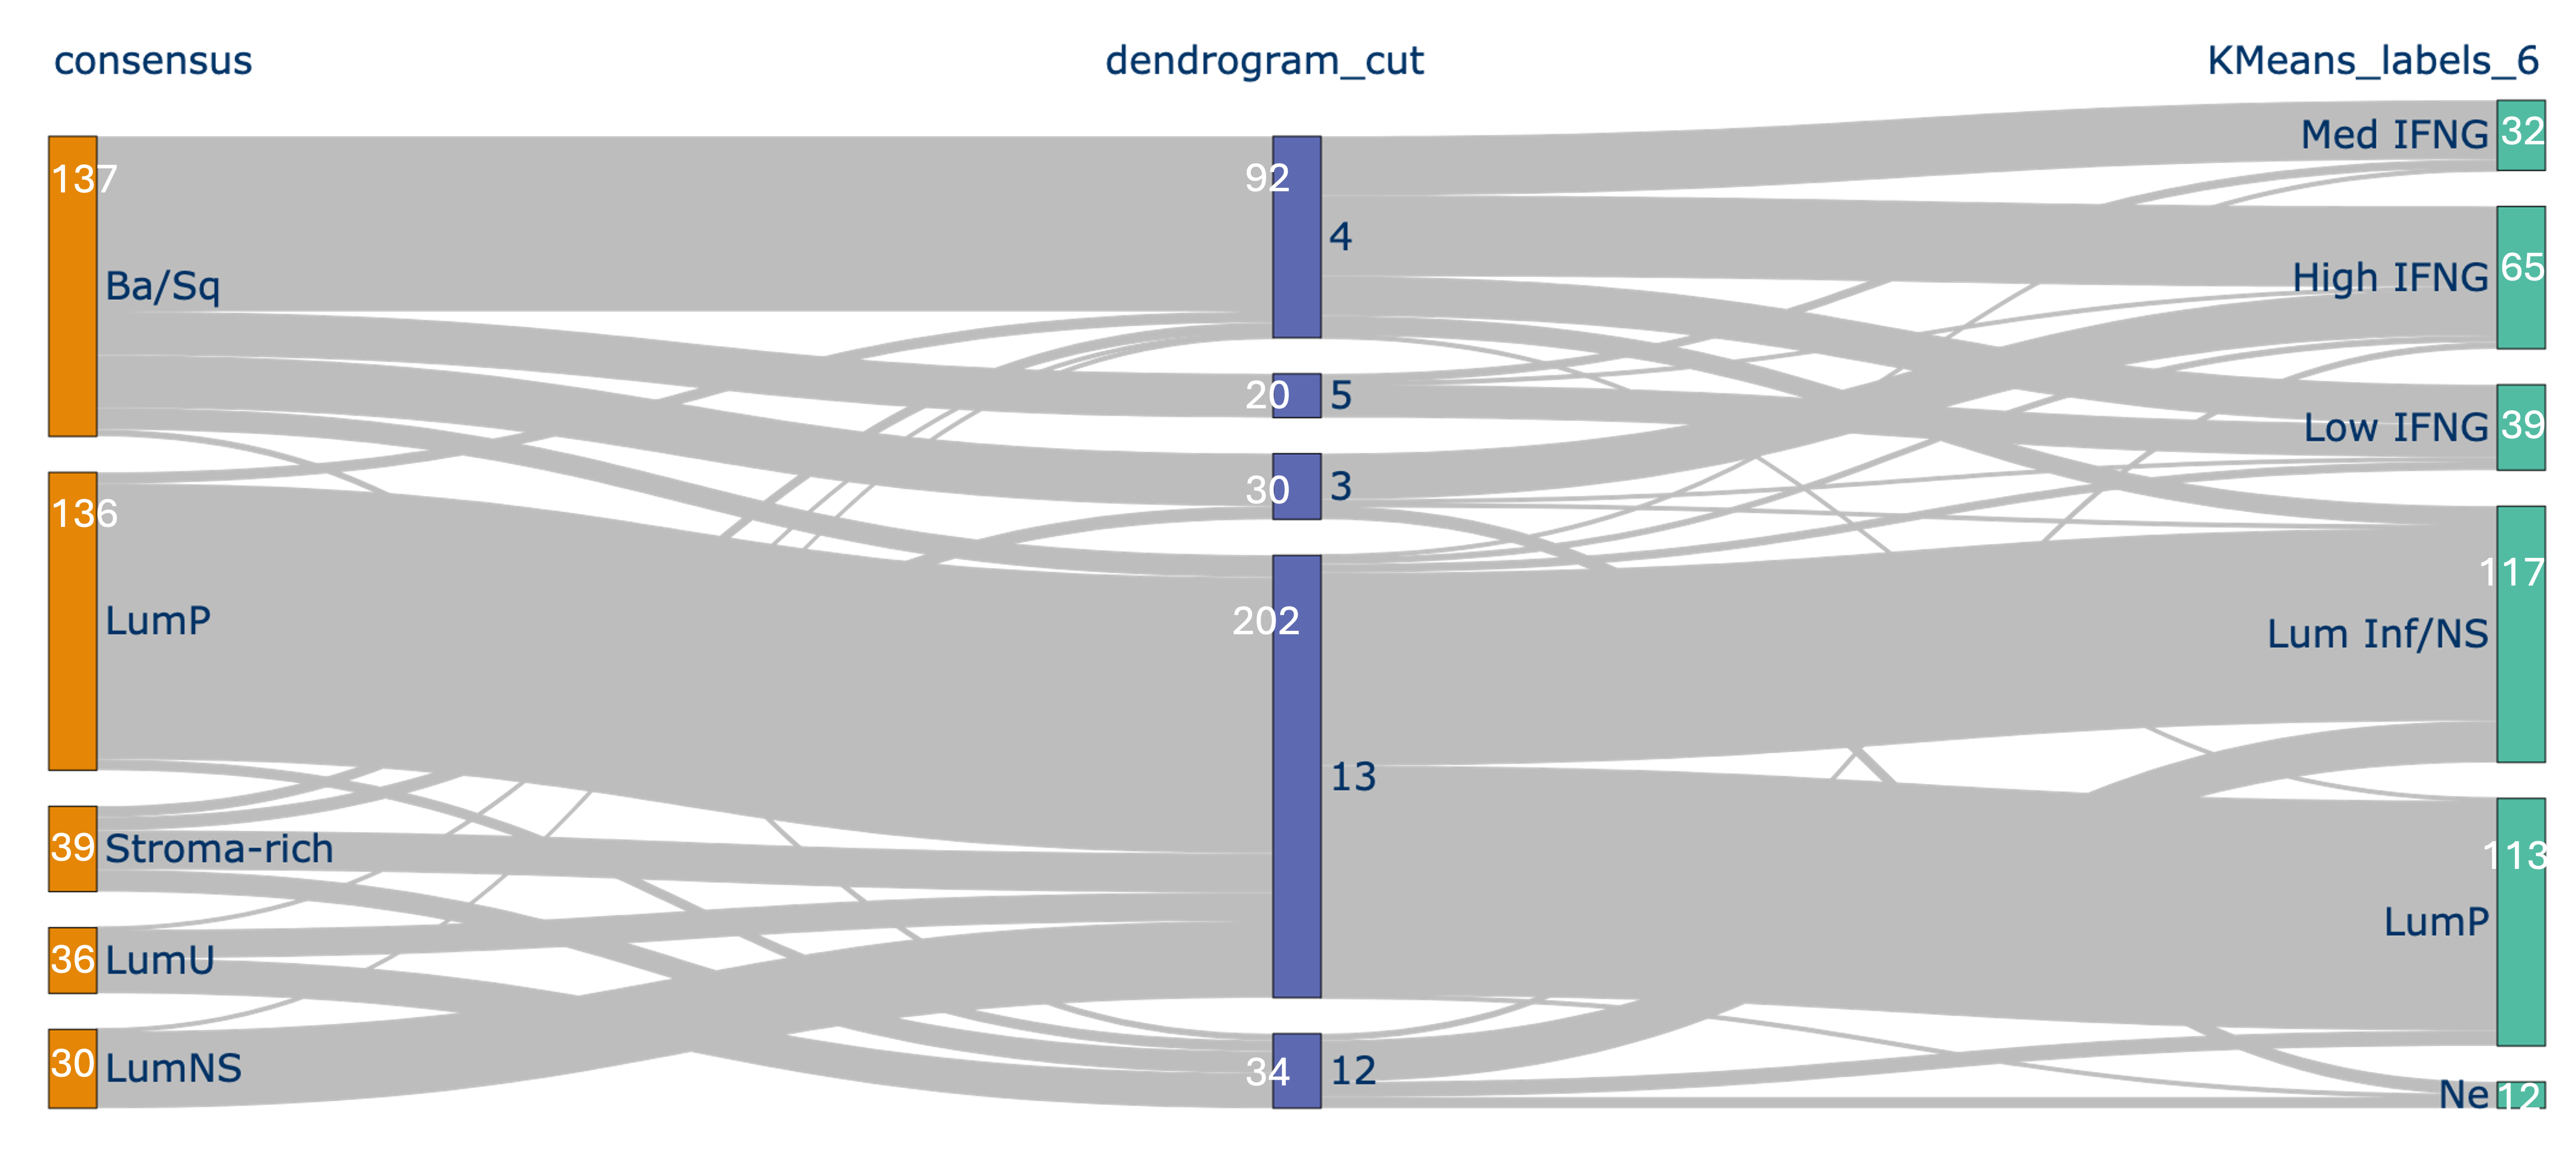
\includegraphics[width=1.0\textwidth,keepaspectratio]{Sections/Network_I/Resources/selective_pruning/sel_tfs/sankey_sel_tfs_VU_CS.png}
        \caption{MIBC groups from 98 TF vs consensus \citep{Kamoun2020-tj} vs the 6 MIBC groups earlier clustering (\ref{s:clustering_analysis}).}
        \label{fig:N_I:sankey_sel_tfs_vuCs}
    \end{subfigure}
    % Sankey - TCGA and Lun comparison  
    \begin{subfigure}[!t]{1.0\textwidth}
        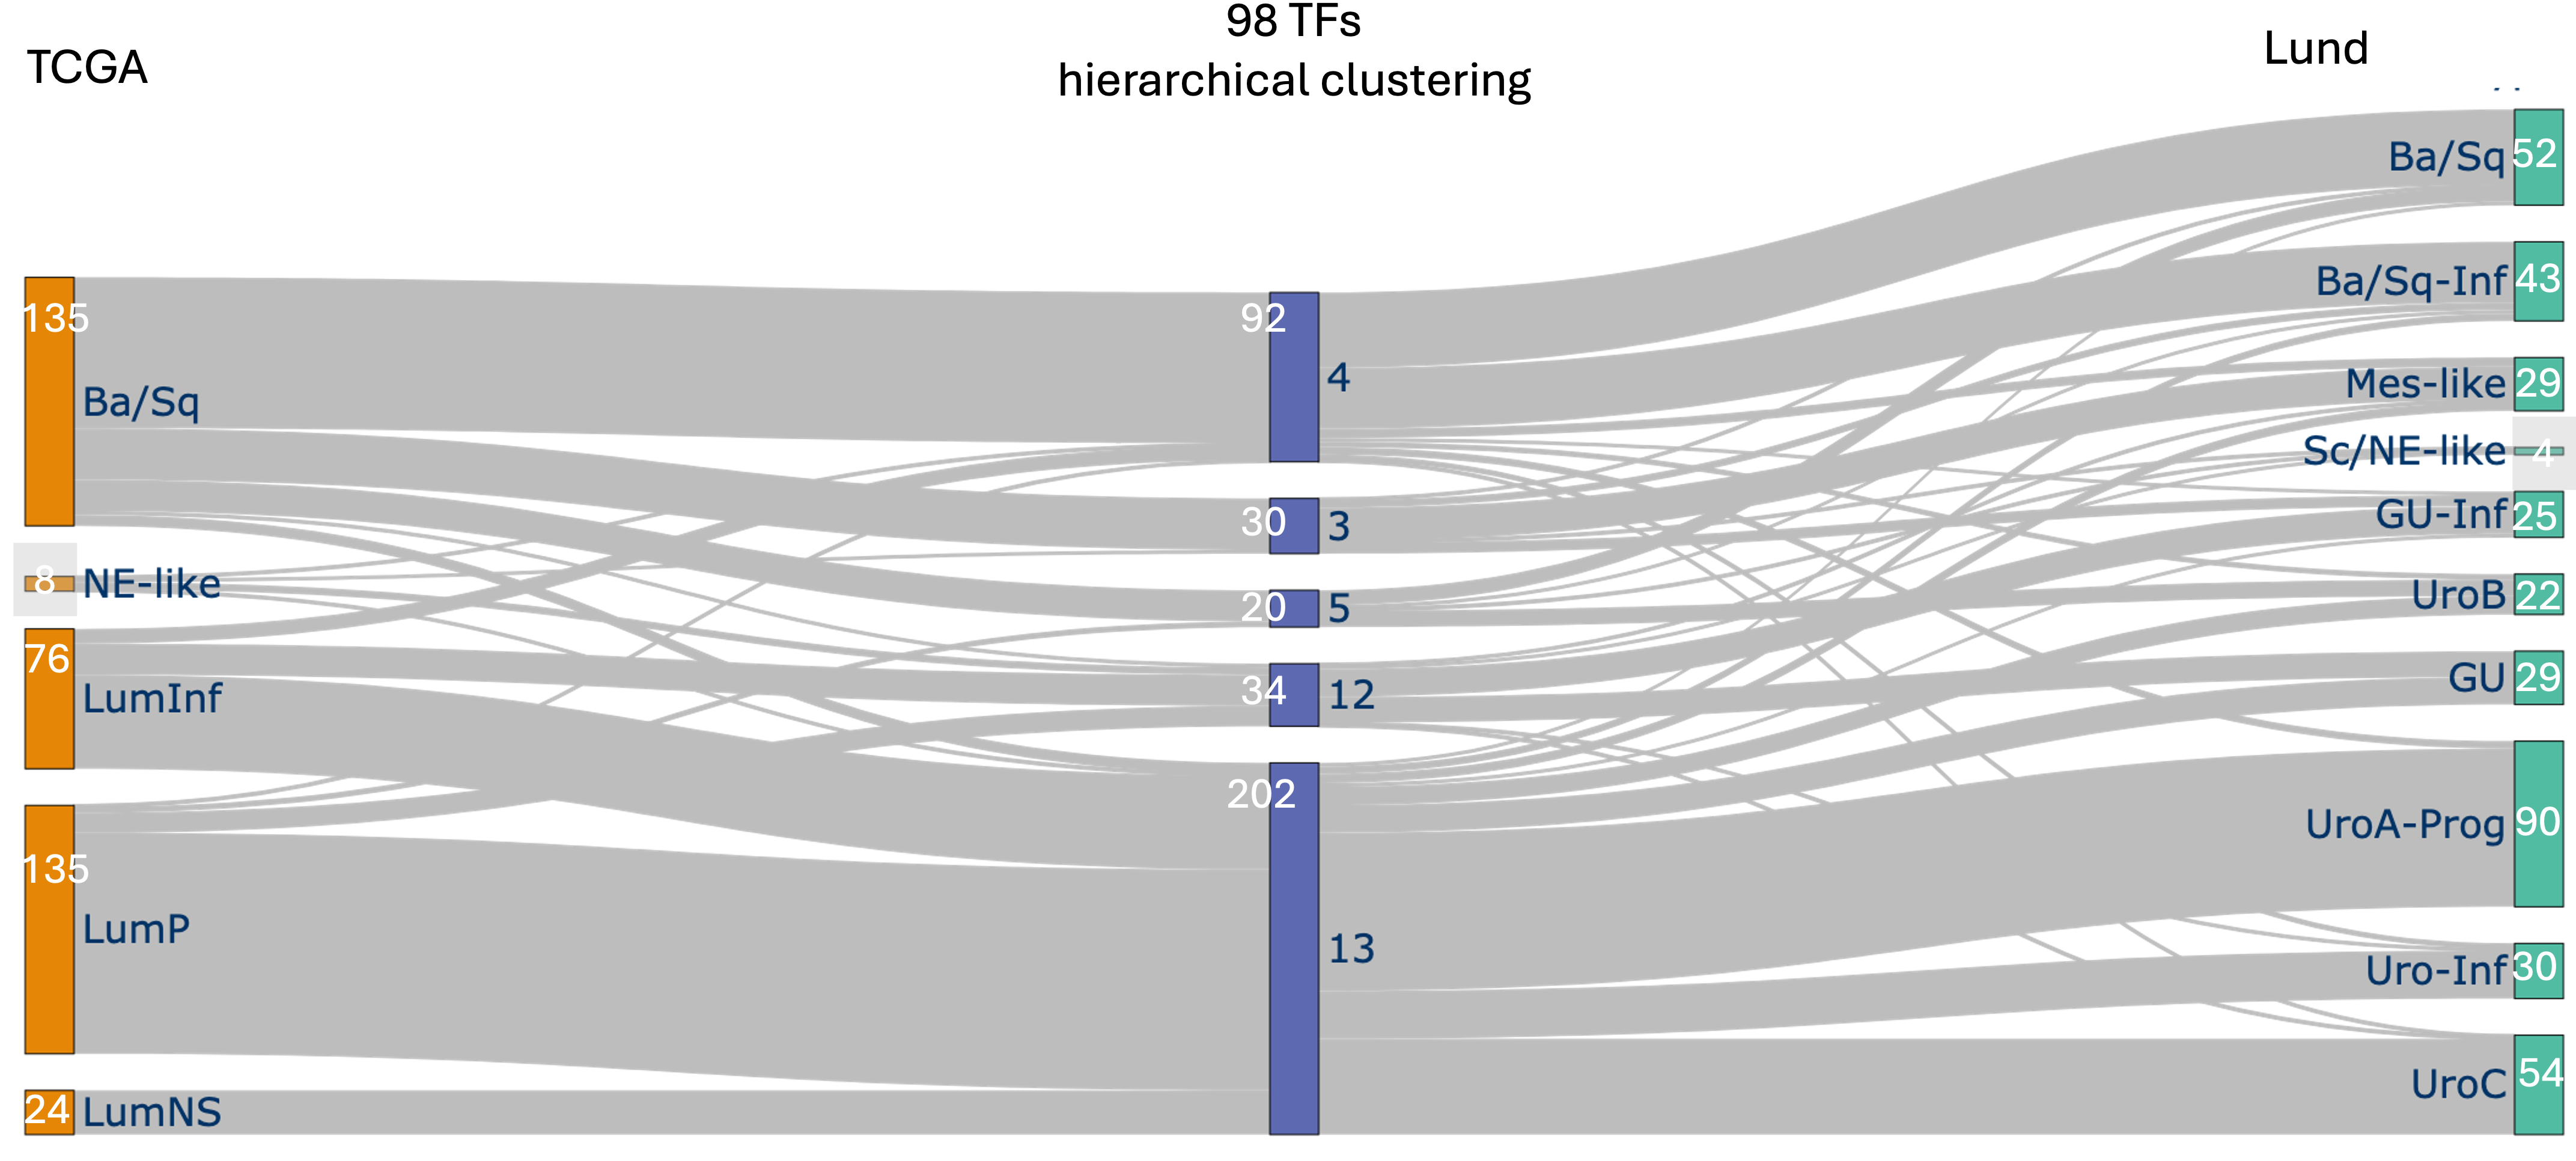
\includegraphics[width=1.0\textwidth,keepaspectratio]{Sections/Network_I/Resources/selective_pruning/sel_tfs/sankey_sel_tfs.png}
        \caption{MIBC groups from 98 TF vs consensus \citep{Kamoun2020-tj} vs Lund \citep{Marzouka2018-ge};}
        \label{fig:N_I:sankey_sel_tfs}
    \end{subfigure}
    \caption[MIBC found from the 98 TF]{Cluster analysis of the subgroups derived using the found 98 TF; see \cref{s:ap:sel_tfs_cs}. The white text on the Sankey plots represents the size of the groups. }
    \label{fig:N_I:sel_tfs_cs_analysis}
\end{figure}


\paragraph*{Basal}

There are three basal subgroups: a main subtype containing most of the previously classified basal samples, group 3, which consists of High IFNG samples, and group 5, which includes Low IFNG samples; see \cref{fig:N_I:sankey_sel_tfs_vuCs}. Based on previous analyses in the project (Basal subtypes from cluster analysis in \cref{s:cs:basal_interp}), group 3 is likely to exhibit a higher immune response compared with groups 5 and 4.

% Comparing with Lund
When comparing these groups with the TCGA and Lund classifiers (\cref{fig:N_I:sankey_sel_tfs}), it is evident that the larger basal group (4) contains most of the Ba/Sq or Ba/Sq-infiltrated samples. The medium-sized group 3 primarily consists of Mes-like samples, while the smaller group 5 comprises UroB and Ba/Sq samples. Notably, the UroB and Low IFNG groups have a poor survival prognosis, whereas the High IFNG samples in group 3 are associated with a more favourable prognosis, as observed in the cluster analysis chapter (\cref{s:clustering_analysis}) and consistent with the Lund classifier \citep{Marzouka2018-ge}.

Overall, the Sankey plots suggest that group 4 is largely composed of Ba/Sq samples, group 3 includes patients classified as Ba/Sq with immune infiltration, and group 5 consists of Ba/Sq samples with no immune response, previously classified as UroB. These findings align with the expected survival outcomes: group 3 is anticipated to have the highest survival rate, group 5 the lowest, and group 4 an intermediate prognosis. This is further confirmed by the Kaplan-Meier survival analysis presented in \cref{fig:N_I:sel_tfs_survival}.

% Luminal groups
\paragraph*{Luminal}

There is a large Luminal group of 202 samples which contains most (83\%), if not all, of the tumour previously classified as LumP, Stroma-rich, LumU, and LumNS (from consensus) and as LumInf/NS and LumP (from KMeans\_6). This is also the case in \cref{fig:N_I:sankey_sel_tfs}, where group 13 contains the LumInf, LumP, LumNS (TCGA) and the UroA-Prog, Uro-Inf, and UroC from Lund. The smaller luminal group (12) consists mostly of the samples from LumU, Stroma-rich from TCGA (\cref{fig:N_I:sankey_sel_tfs_vuCs}) or the consensus LumInf/LumP (TCGA) or the Genomically Unstable (GU) and GU-infiltrated from Lund.

% Summary of the comparison
The comparison with the other stratification methods shows that clustering the expression of 98 TF is capable of finding three basal subtypes, two smaller even than the ones found in the previous cluster analysis from \cref{s:clustering_analysis}. However, the 98 TF fail to discriminate between luminal subgroups.

% Survival analysis
\subsection{Survival Analysis}

The Kaplan-Meier Survival analysis was conducted on the five groups derived from the 98 transcription factors as shown in \cref{fig:N_I:sel_tfs_survival}. Group 5, identified as the smallest basal group, exhibits the poorest survival prognosis by a significant margin. Notably, the poorest survival in both the TCGA and consensus classification is observed in the Neuroendocrine-like groups, which are not included in Group 5; see Sankey plot in \cref{fig:N_I:sankey_sel_tfs}. It is striking the poor survival of the group 5, where almost all of the patients are deceased after 3 years, it has a worst survival even then the UroB group from the Lund classifier (see survival plot in \cref{fig:N_I:sel_tfs_comp_leiden}) and the Low IFNG Basal from \cref{s:cs:basal_interp}.

The largest luminal group (13) demonstrates the most favourable prognosis, followed by the medium-sized basal cluster, basal 4 (3). Basal group 3 exhibits the best survival rate at the five-year mark compared to the other two basal groups (4 and 5), though the difference between groups 3 and 4 is not as pronounced as initially hypothesised. The luminal infiltrated group (12) shows survival trends similar to clusters 3, 4, and 13, but its survival prognosis deteriorates over the five-year period. The multivariate log-rank test, yielding a $p<0.005$, confirms the statistical significance of the differences in survival among the five groups.


% Giving context to the results
The clustering analysis shows that the by only using 98 genes, the main groups, Basal and Luminal, are discovered. The survival analysis indicates that these subtypes have significantly different survival prognosis. The gene expression heatmap from \cref{fig:ap:morph_sel_tfs} reveals that there some highly varied genes\footnote{This is given by the rows that are either completely blue or red (\textit{BNC1, FOXJ3, ELF3}), suggesting that there }, which are later confirmed by the bar plot from \cref{fig:N_I:sel_tfs_var}. 


\begin{figure}[!t]
    \centering
    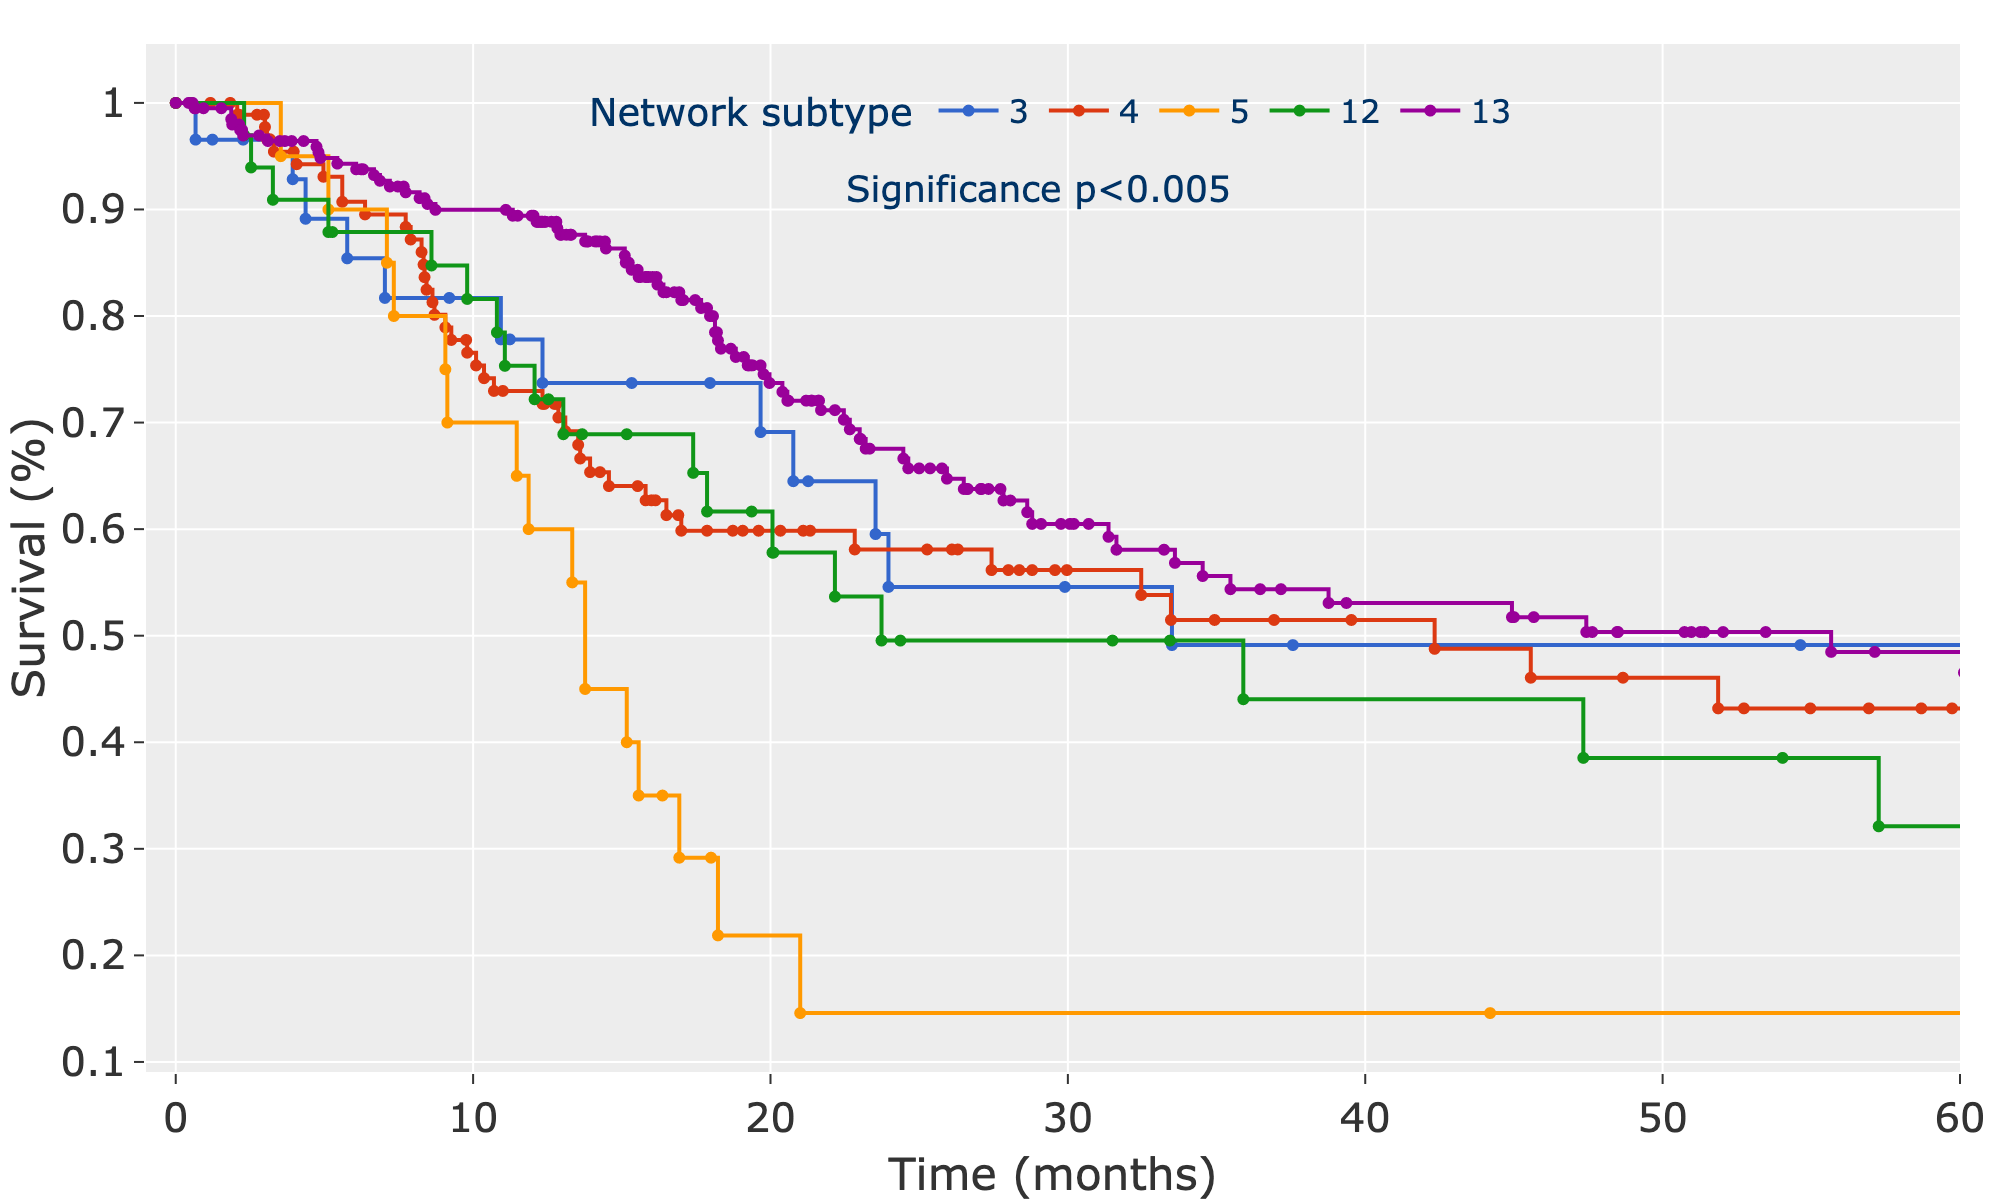
\includegraphics[width=1.0\textwidth,keepaspectratio]{Sections/Network_I/Resources/selective_pruning/sel_tfs/survival_sel_tfs_cs.png}
    \caption[Survival analysis of the five MIBC groups found using the 98 TF]{Kaplan-Meier survival analysis of the MIBC subtypes derived from the expression of the 98 TF. The multivariate long rank test found a significant difference of 0.000140 between the survival of the five groups. Group 5 have one of the lowest survival prognosis seen in the literature. }
    \label{fig:N_I:sel_tfs_survival}
\end{figure} 


\subsubsection*{Comparing with other classifications} \label{s:N_I:sel_tfs_comp_survival}

The comparison with the Lund classification \citep{Marzouka2018-ge} revealed that the three basal groups, 3, 4, and 5, include many samples previously classified as Mes-like, Ba/Sq, and UroB. To assess the novelty of the subtypes identified using the 98 TF, the survival rates of these three groups were compared between the two classifications, as shown in \cref{fig:N_I:sel_tfs_comp_leiden}.

Group 5 and UroB exhibit similar trends but are significantly different (p: 0.0269), with Group 5 consistently showing a worse prognosis, with less than 20\% chance of survival after two years of the prognosis. Samples in Basal 4 demonstrate more favourable survival rates overall, while the two Mes-like subgroups display comparable trends. Overall, the survival analysis comparison indicates that the three Basal groups identified using the 98 TF align closely with the corresponding subtypes from the Lund classifier. This also highlights the effectiveness of the 98 TF in identifying these subgroups without the need for \acrlong{ihc}, as was required in the Lund classifier.

Performing a similar comparison of the three basal groups with the subtypes from TCGA \citep{Robertson2017-mg}, there are significant differences (p: 0.06) between the two classifications. Basal 5 exhibits a worse prognosis than the tumours classified as Ne.

Compared with the project's earlier work on clustering analysis, the Basal 5 group contains 15 samples previously classified as Low IFNG, four as Medium IFNG, and one as High IFNG. When comparing the survival trends, the basal groups found using the 98 TFs exhibit significant differences (p: 0.002674) from the subtypes found using clustering analysis. This indicates that there is a subgroup of Basal groups that have a poor prognosis with aggressive markers.

\begin{figure}[!htb]
    \centering
    % Sankey - consensus and K-means comparison
    \begin{subfigure}[!t]{1.0\textwidth}
       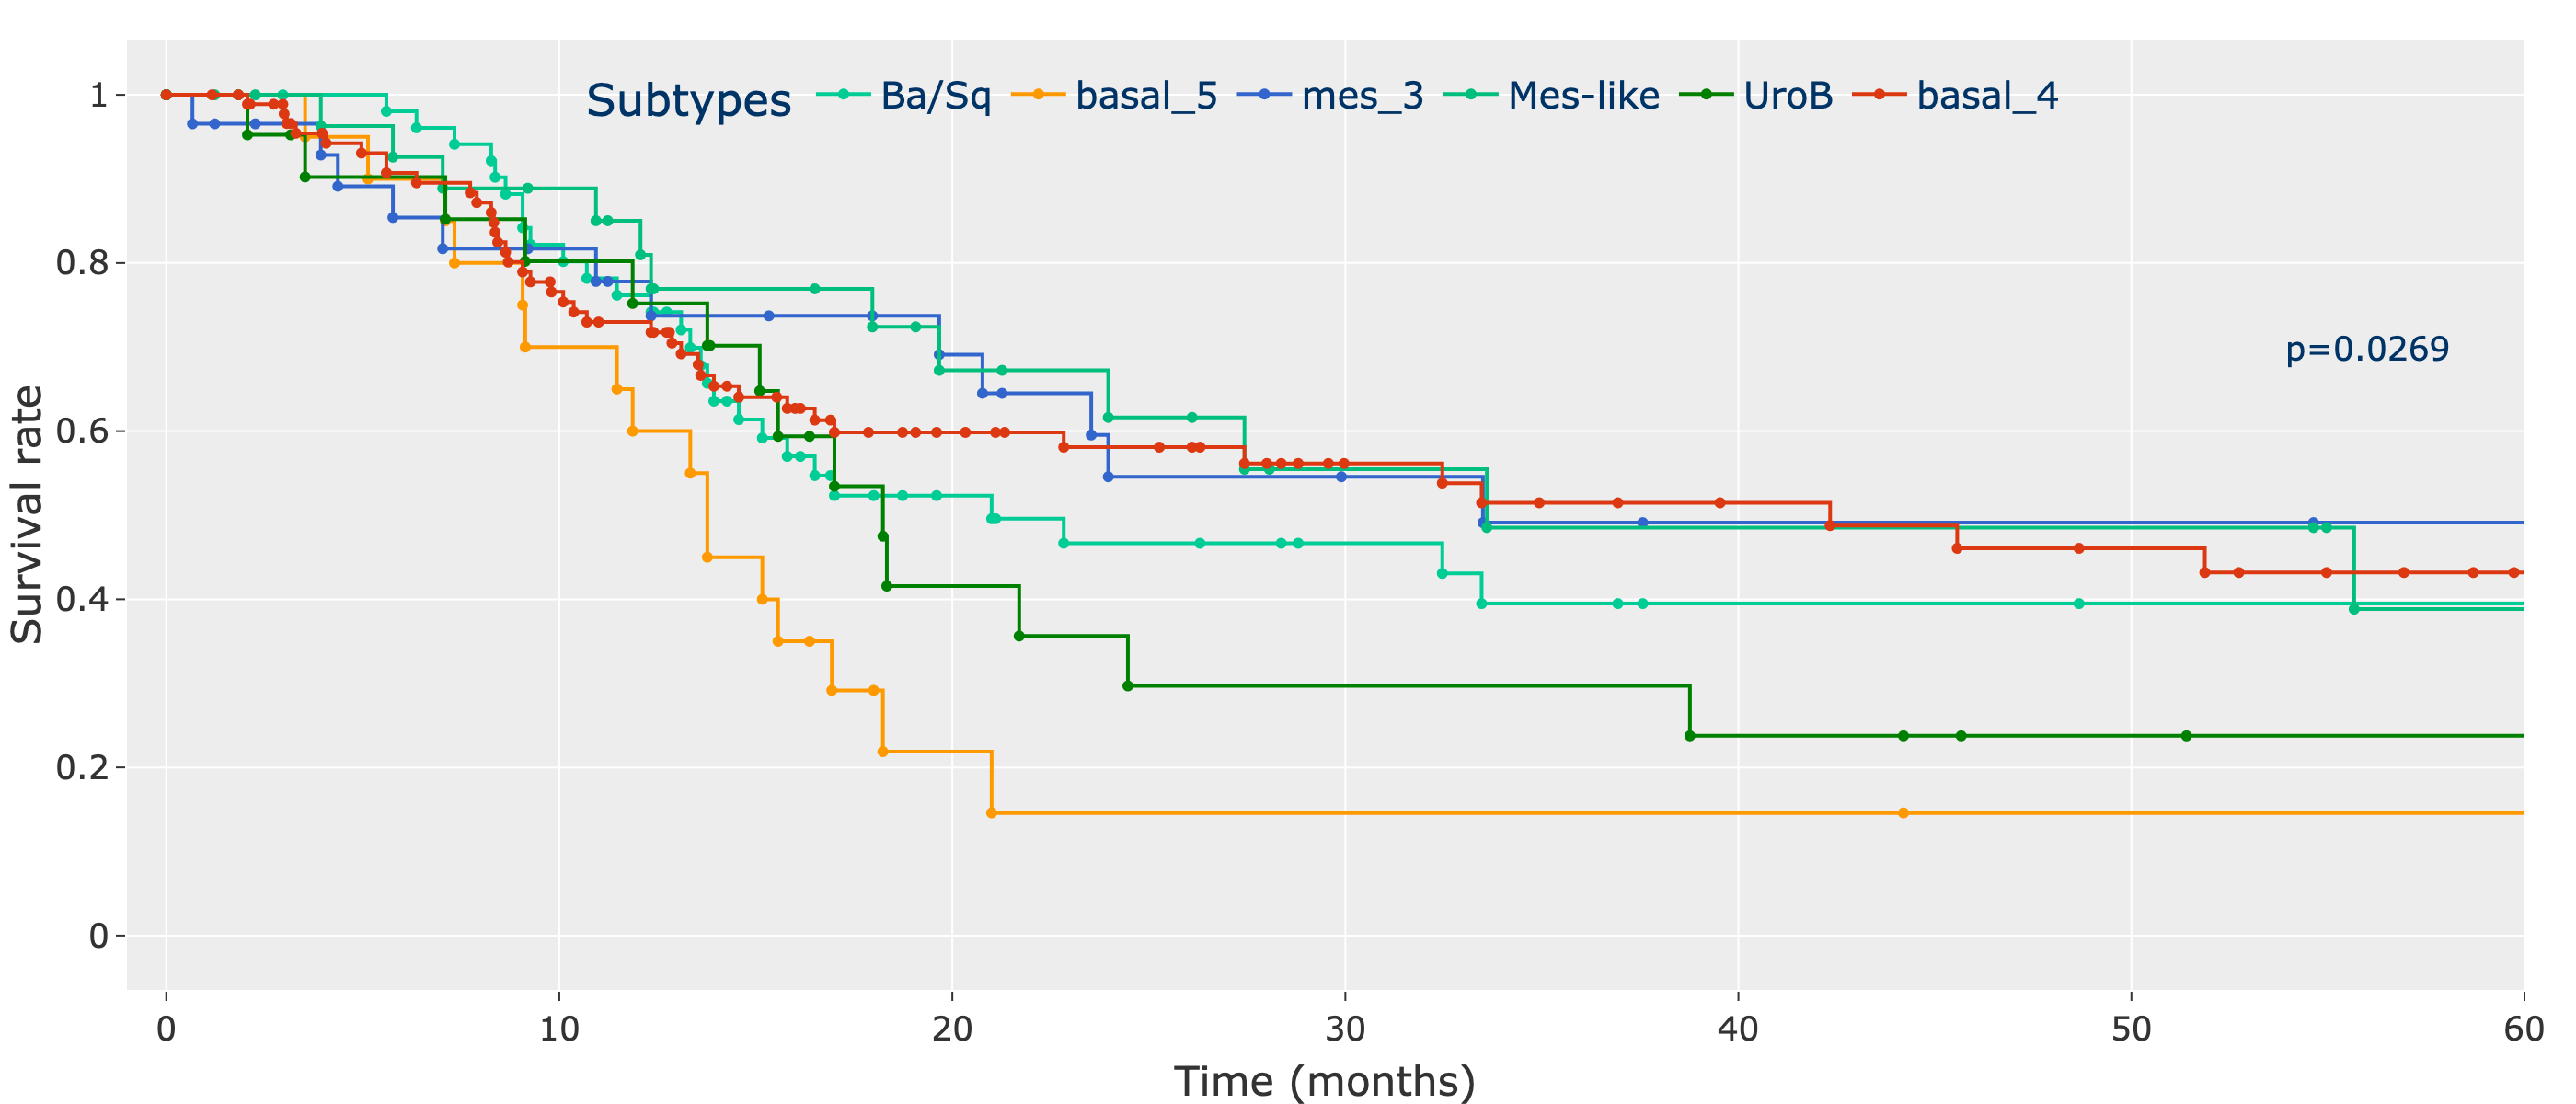
\includegraphics[width=1.0\textwidth,keepaspectratio]{Sections/Network_I/Resources/selective_pruning/sel_tfs/comp_leiden_survival.png}
        \caption{Lund}
        \label{fig:N_I:sel_tfs_comp_leiden}
    \end{subfigure}
    % Sankey - TCGA and Lun comparison  
    \begin{subfigure}[!t]{1.0\textwidth}
        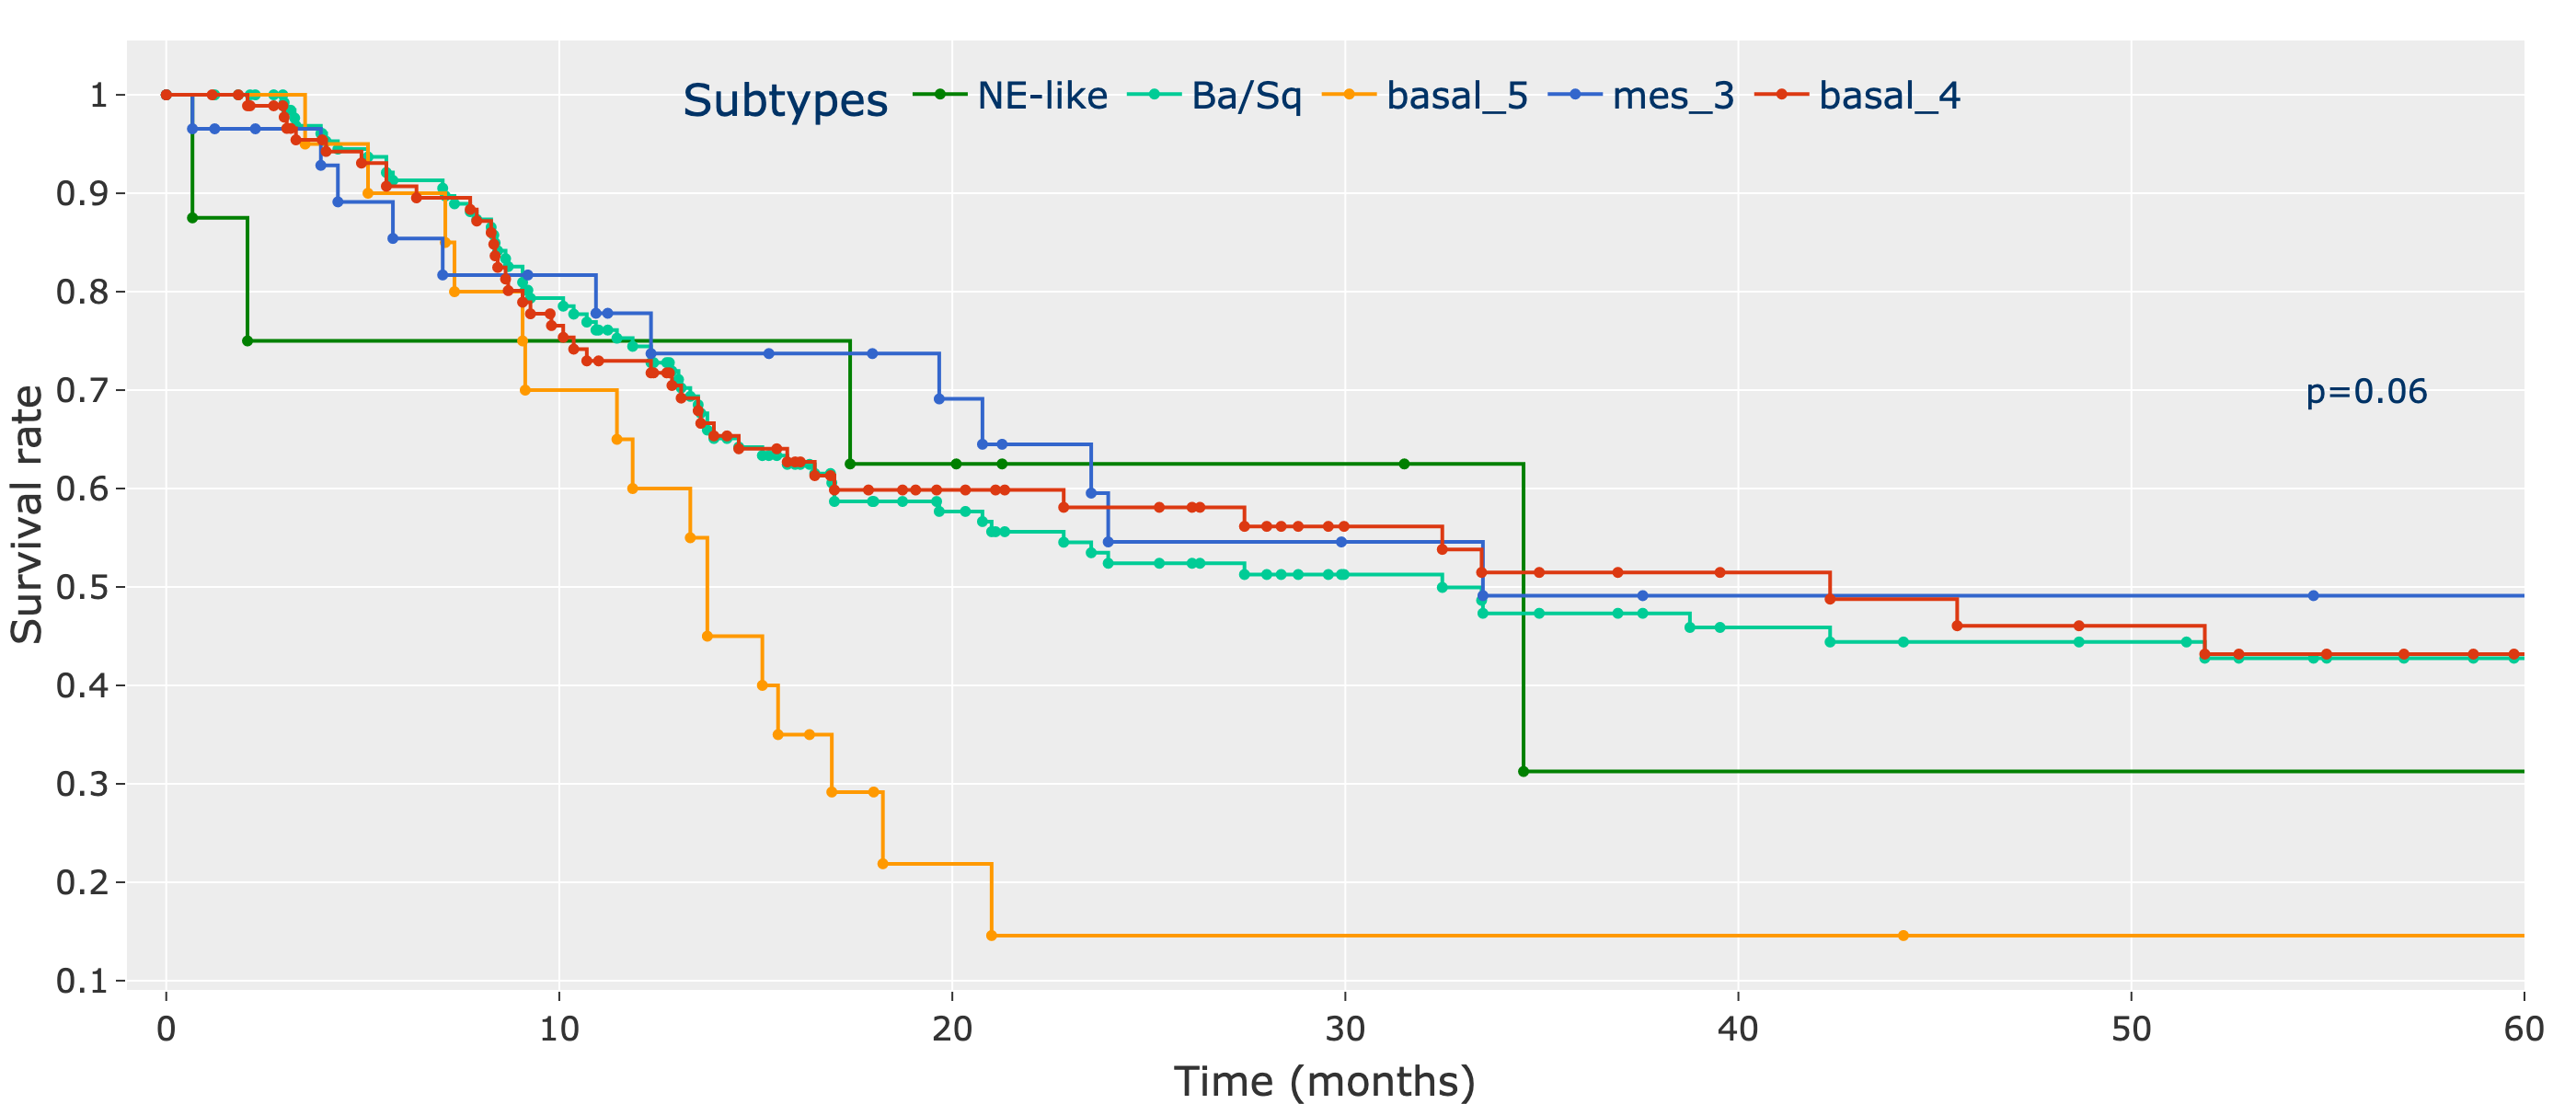
\includegraphics[width=1.0\textwidth,keepaspectratio]{Sections/Network_I/Resources/selective_pruning/sel_tfs/comp_leiden_survival_tcga.png}
        \caption{TCGA}
        \label{fig:N_I:sel_tfs_comp_tcga}
    \end{subfigure}
    \begin{subfigure}[!t]{1.0\textwidth}
        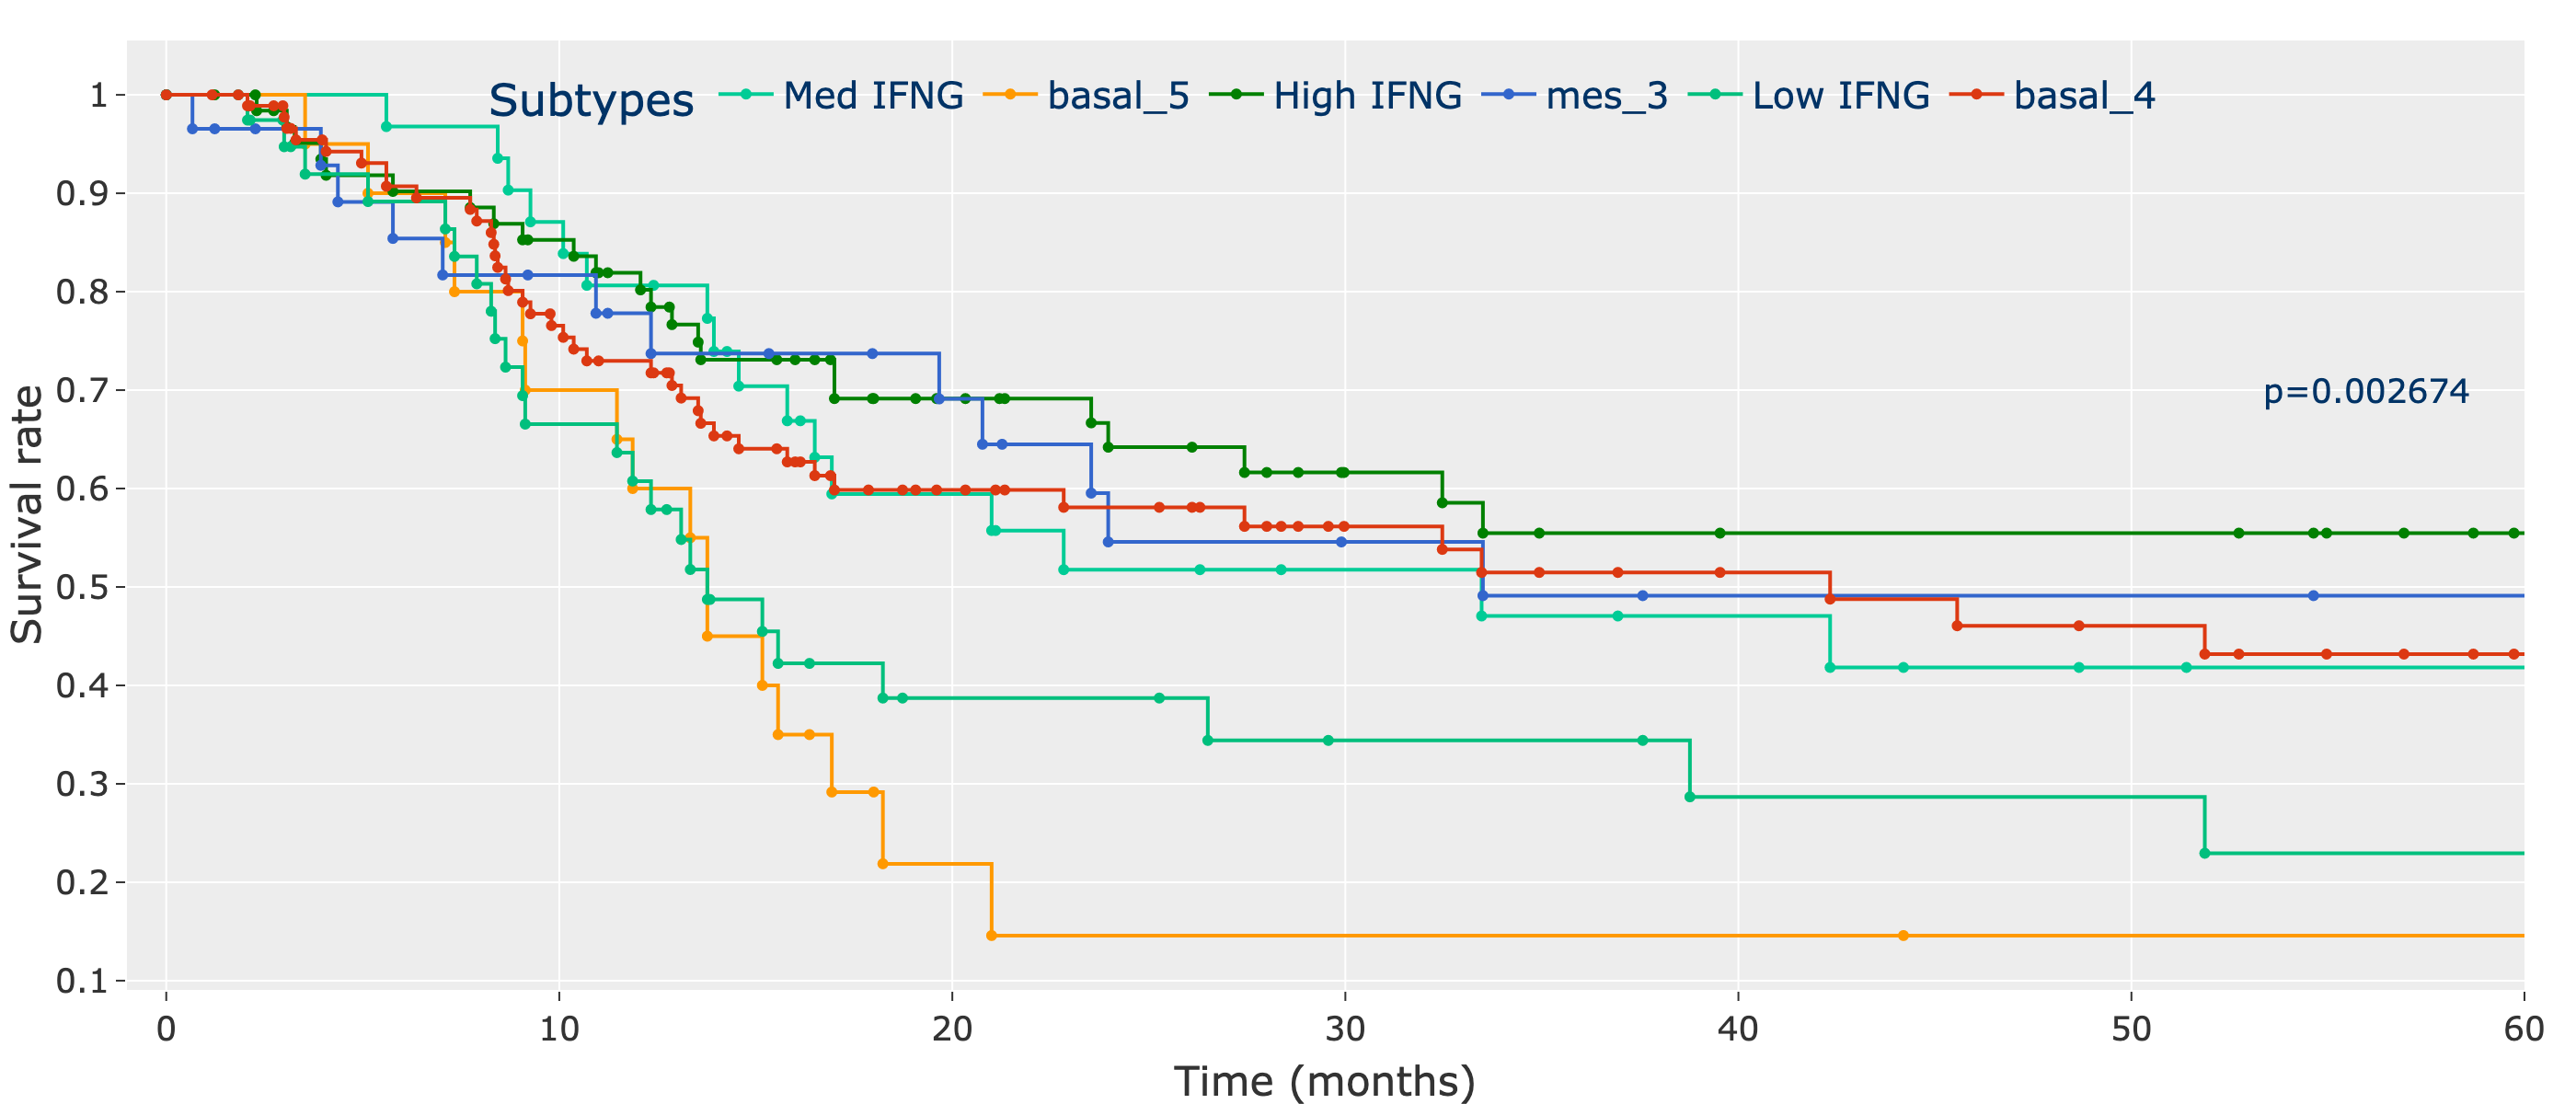
\includegraphics[width=1.0\textwidth,keepaspectratio]{Sections/Network_I/Resources/selective_pruning/sel_tfs/comp_leiden_survival_CA.png}
        \caption{Clustering Analysis}
        \label{fig:N_I:sel_tfs_comp_CA}
    \end{subfigure}
    \caption[Survival comparison with TCGA, Lund and CA]{Kaplan-Meier survival analysis of the three basal groups 3, 4 and 5, compared with selected groups from Lund classification \citep{Marzouka2018-ge}, TCGA \citep{Robertson2017-mg} and cluster analysis \cref{s:clustering_analysis}. The survival comparisons shows that the MIBC groups found using the 98 TFs consistently exhibit significantly different survival prognosis compared to the others. See \cref{s:N_I:sel_tfs_comp_survival}.}
    \label{fig:N_I:sel_tfs_cs_comp}
\end{figure}

% \begin{figure}[!htb]
%     \centering
%     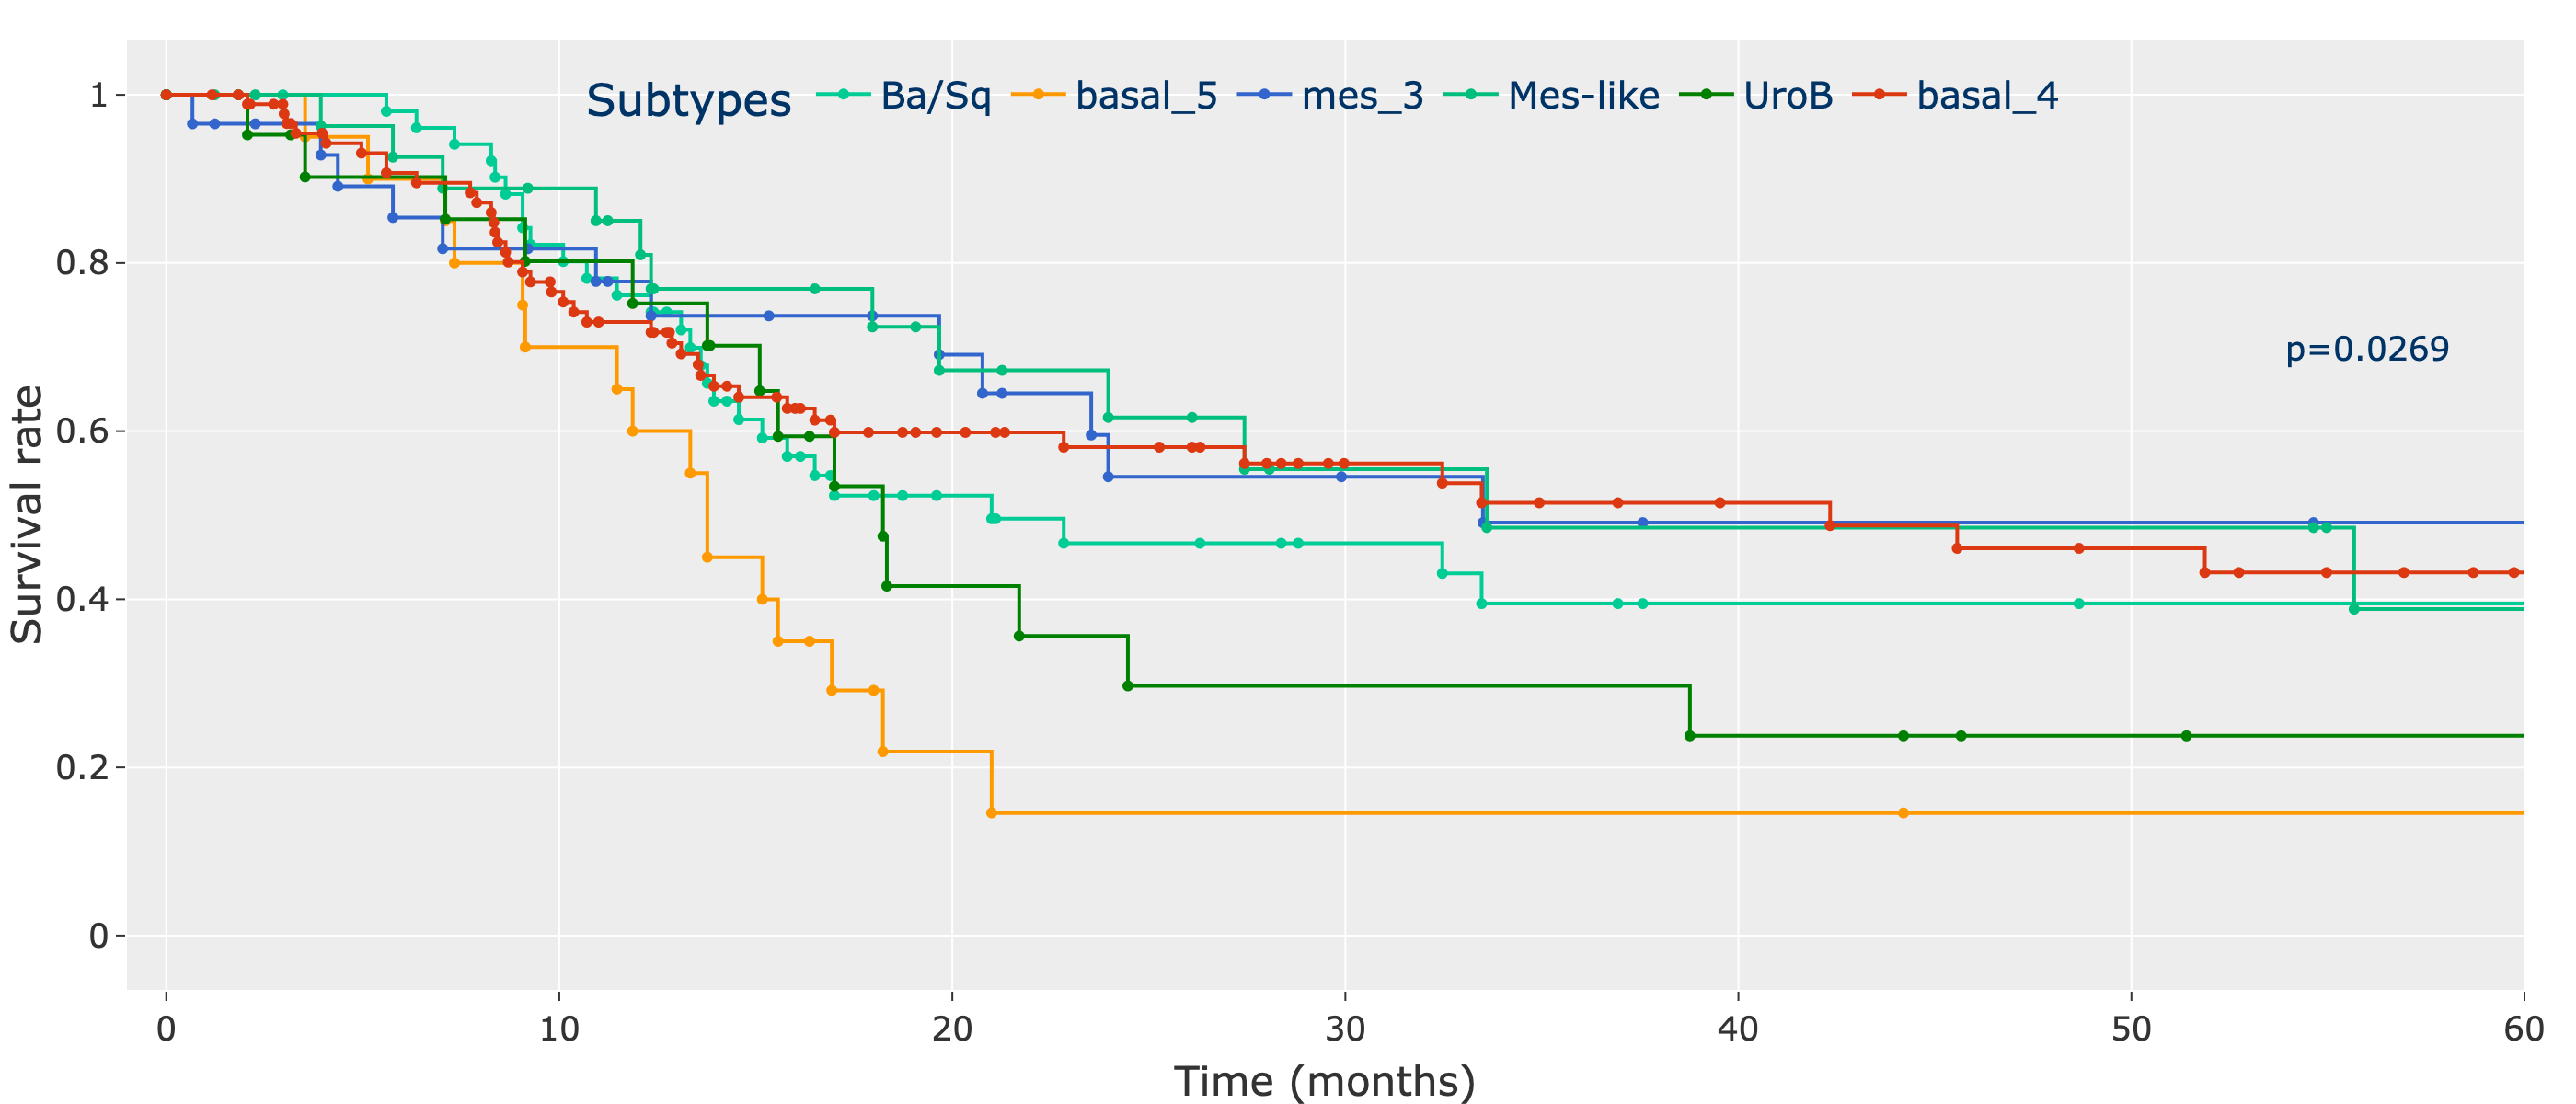
\includegraphics[width=1.0\textwidth,keepaspectratio]{Sections/Network_I/Resources/selective_pruning/sel_tfs/comp_leiden_survival.png}
%     \caption[Basal 5 and UroB low survival prognosis]{Kaplan-Meier survival analysis of the three basal groups 3, 4 and 5, compared with Ba/Sq, UroB and Mes-like groups from Lund classification \citep{Marzouka2018-ge}. The survival comparison showing the similar trends in prognosis of the groups found using 98 TF and the subtyps derived using \citet{Marzouka2018-ge} which used gene expression and \acrlong{ihc} data. }
%     \label{fig:N_I:sel_tfs_comp_leiden}
% \end{figure} 




% Varying expressiong across subgroups
\subsection{Varying expression across subgroups} \label{s:N_I:sel_tfs_ge}

% Introduce of the plots
The dumbbell figure in \cref{fig:N_I:dumbell_sel_tfs} exhibits the difference in expression between subgroups. Each point represents the $log2(mean\_TPM+1)$, and the subplots are in descending order of the fold change between the averages of the two groups.

% Basal and Luminal signal
The expression differences between groups 4 and 13 show the basal/luminal difference in the gene expression of the 98 TF, where the largest change is on \textit{BNC1} is expressed in the basal group but not in the luminal; see plot A from \cref{fig:N_I:dumbell_sel_tfs}. Known differentiation markers are also present, which include genes like \textit{GRHL3} \citep{Ramal2024-ha} or \textit{MYCL}.

% BNC1
Plot B shows that groups 13 and 12 have similar expressions in the 98 TF, with cluster 13 having a considerably higher expression in the \textit{TP63}. \Cref{fig:N_I:dumbell_sel_tfs} A) and C) shows that \textit{BNC1} is absent in both Luminal groups. This gene is also lowly expressed in the basal subtypes in comparison with the mes-like group in D) and E). \textit{BNC1} is a squamous cell marker as shown by the work of \citet{Hurst2022-sp}

% Basal 5 and Luminal 13 and Mes-like
Group 5 is formed out of mostly samples (15) from the Low IFNG group from previous clustering analyses (\cref{s:cs:basal_interp}), tissues which did not exhibit an \acrlong{ifn} response. Group 12 has a large proportion of samples that were previously classified as luminal infiltrated, and group 3 consists mostly of mes-like samples. Comparing the two with the basal group shows that the latter exhibit more Basal/Squamous markers or \textit{TP63} or \textit{BNC1}.


\begin{table}[!t]
    \centering
    \scriptsize
    \begin{tabularx}{\textwidth}{>{\hsize=0.8\hsize}X|>{\hsize=0.8\hsize}X|>{\hsize=1.4\hsize}X}
        \toprule
        \textbf{Comparison} & \textbf{Differences in expression} & \textbf{Remarks} \\
        \midrule
        Basal 4 and Luminal 13 (A) & \textit{BNC1, MYCL, FOXQ1, HES2, GRHL3, HOXB6} & Shows the difference in the two main MIBC groups: Basal and Luminal \\
        \midrule
        Luminal 13 and Luminal infiltrated 12 (B) & \textit{TP63}; no expression of \textit{BNC1} & Similar groups both lack expression of the squamous marker \textit{BNC1} \\
        \midrule
        Basal 5 and Luminal infiltrated 12 (C) & \textit{TP63, BNC1, HES2, MSX2, MYCL, HOXB6, IRF6, GRHL3} & Squamous markers (\textit{TP63, BNC1}) higher expressed in Basal 5 \\
        \midrule
        Mes-like 3 and Luminal 13 (D) & \textit{TP63, MYCL, GRHL3, ELF3, BNC1, ZNF750, ZBTB7C, MYCL} & Ba/Sq markers \textit{(TP63, ZBTB7C, BNC1)} more pronounced in the Mes-like 3 group over the Luminal \\
        \midrule
        Mes-like 3 and  Basal 5 (E) & \textit{GRHL3, TP63, HES2, IRF6, ZBTB7C, ZNF750, BNC1, OVOL1} & Ba/Sq markers (\textit{TP63, ZBTB7C, BNC1}) more pronounced in Basal 5 \\
        \midrule
        Basal 4 and 5 (F) & \textit{ZBTB7C, MECOM, MSX2, TP63, KLF5, ELF3} & The Ba/Sq markers are stronger in the Basal 5 \\
        \bottomrule
    \end{tabularx}
    \caption[Summary of the gene expressions]{Summary of the gene expression comparisons from \cref{fig:N_I:dumbell_sel_tfs}. The main takeaway is that the Basal groups 4 and 5 exhibit Ba/Sq markers with strong expression.}
    \label{tab:N_I:dumbel_summarry}
\end{table}

% Squamous signal in basal 5
\textit{TP63, ZBTB7C, BNC1} are known Squamous marker \citep{Robertson2023-na,Fishwick2017-kd} and indirectly of the bladder tissue un-differentiation status. The expression of this markers are specific to the two basal groups 4 and 5 as well as to the Mes-like group; see C-F in \cref{fig:N_I:dumbell_sel_tfs}.  Over the three groups, the Basal 5 exhibit the strongest differences as seen in the comparison in E with mes-like and F with the basal 4. It is worth noting, that there is little change in the \textit{TP63} expression in the basal and luminal comparison from A. 

Overall, there are a few genes that have noticeable gene expression across the subgroups derived using the 98 TF which are summarised in table below \cref{tab:N_I:dumbel_summarry}.

% \begin{figure}[!ht]   
\begin{sidewaysfigure}

    \centering
    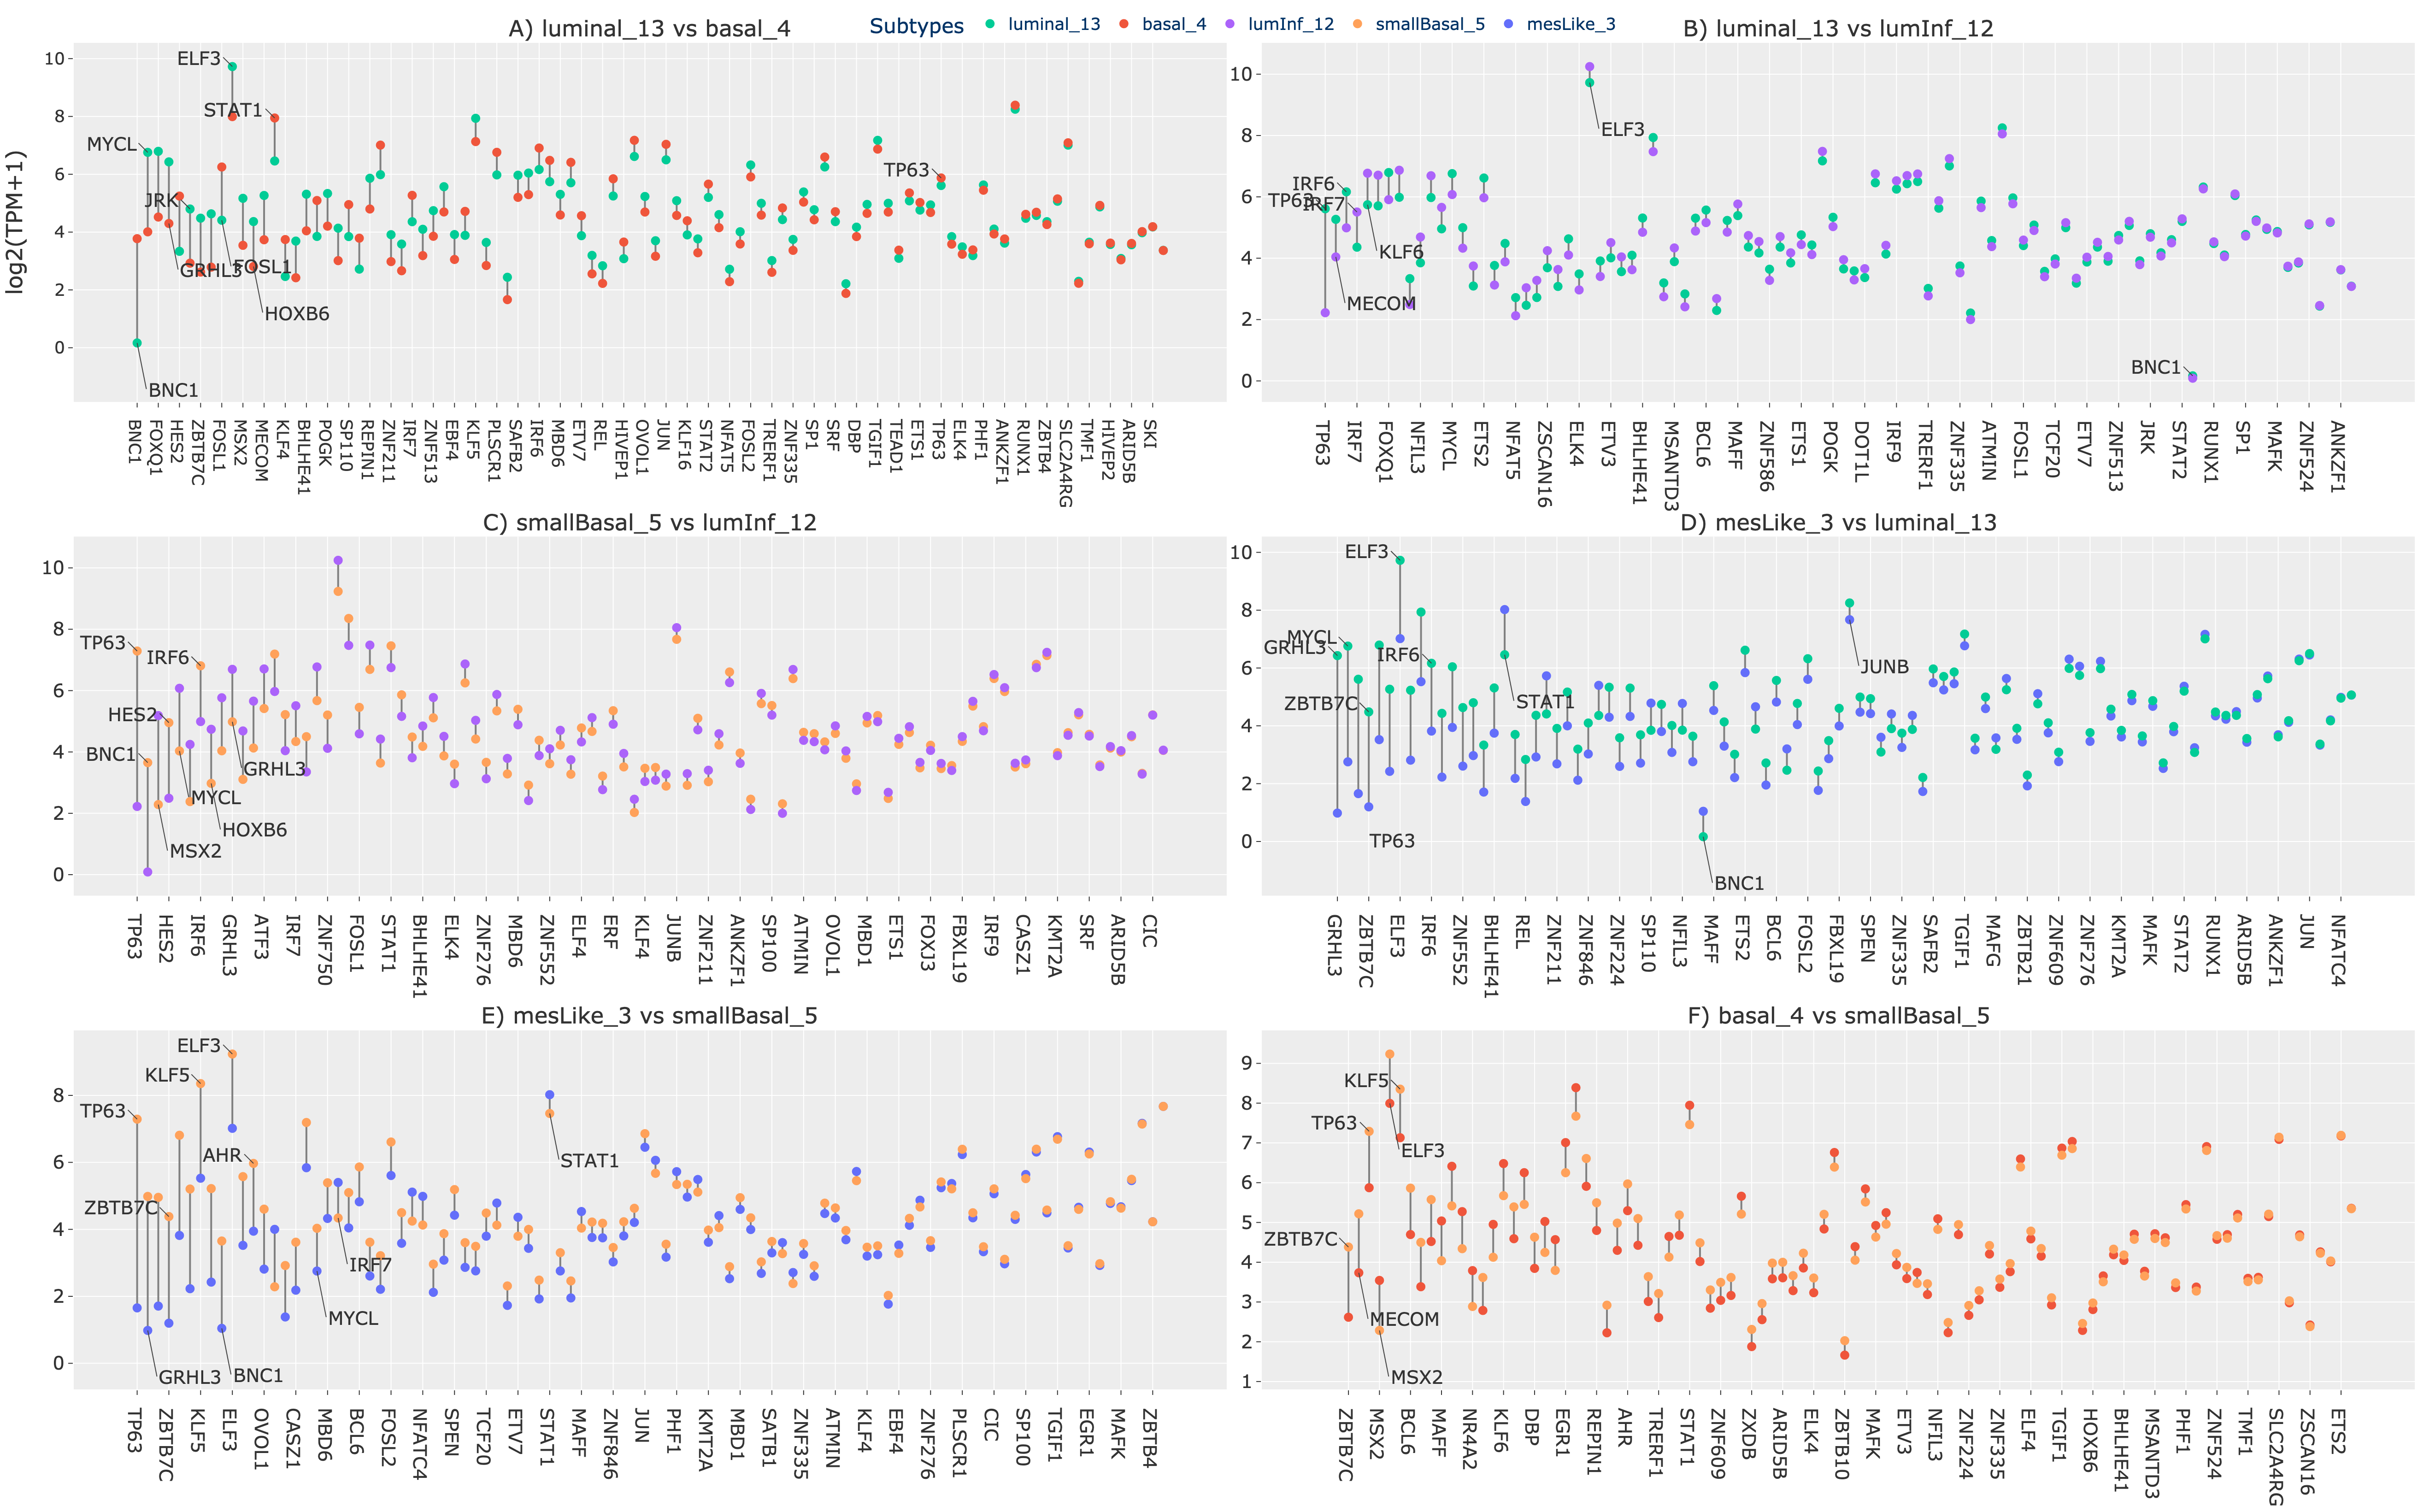
\includegraphics[width=1.0\textwidth,keepaspectratio]{Sections/Network_I/Resources/selective_pruning/dumbell_sel_tfs.png}
      \caption[Mean gene expression acros the five MIBC subgrouos]{Comparison of the mean across the subtypes derived with the 98 TF. Each point represents the $log2(mean\_TPM+1)$ and the subplots are in descending order of the fold change.}
    \label{fig:N_I:dumbell_sel_tfs}
\end{sidewaysfigure}


\subsection{Summary}

This preliminary analysis of the highly connected 98 TF genes reveals a significant survival difference between the groups derived from the analysis, with the Basal 5 group showing the poorest survival prognosis observed in this project. This is a novel finding, as the Basal 5 group consists exclusively of samples previously classified as Ba/Sq \citep{Kamoun2020-tj,Robertson2017-mg}, without any Neuroendocrine samples, which are typically associated with the poorest prognoses. Additionally, the UroB group from the Lund classifier \citep{Marzouka2018-ge} exhibits a similarly poor survival rate, though the Basal 5 group has the worst prognosis.

The preliminary gene expression analysis shown in \cref{fig:N_I:dumbell_sel_tfs} indicates that the Basal 5 group exhibits strong squamous markers. The subsequent section aims to refine the list of 98 TF and investigate the underlying biology of each MIBC subtype.




